

\begin{figure}[h!]
	\centering
	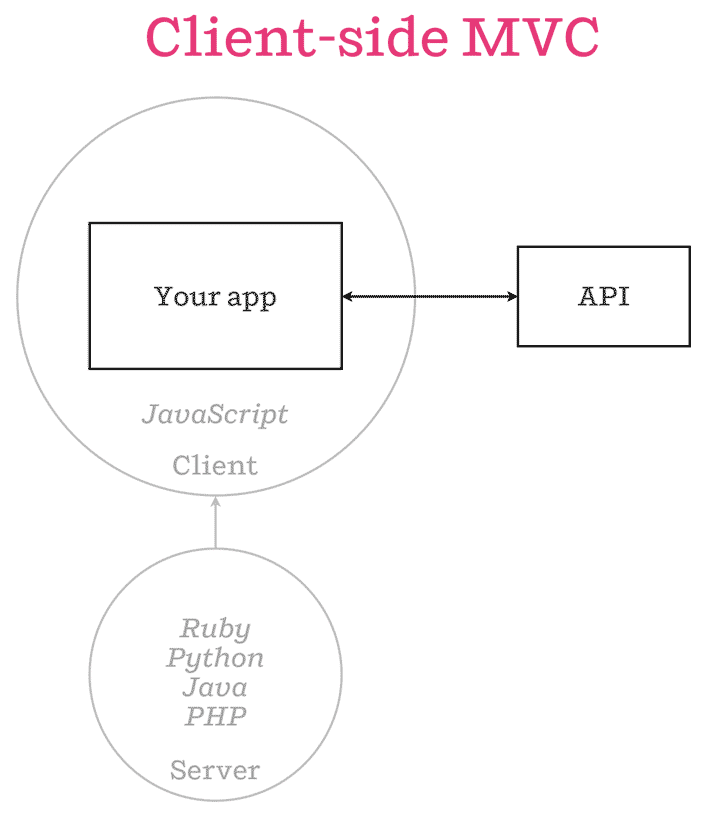
\includegraphics[width=0.5\textwidth]{figuras/estadoArte/isomorphic-client-side-mvc.png}

	\caption{\clientSideAS \mvcAS.}
	\label{figure:client_side_mvc}
\end{figure}

% Definition of circles
\def\firstcircle{(0,0) circle (2)}
\def\secondcircle{(0,-5) circle (1)}

\def\firstrectangle{(-1.5,1) rectangle (1.5,-1)}

\def\secondrectangle{(4,0.5) rectangle (6.5,-0.5)}

\colorlet{circle edge}{blue!50}
\colorlet{circle area}{blue!20}

\tikzset{filled/.style={fill=circle area, draw=circle edge, thick},
    outline/.style={draw=circle edge, thick}}

\setlength{\parskip}{5mm}
% Set A and B
\begin{tikzpicture}
    \begin{scope}
        \clip \firstcircle;
        \fill[filled] \secondcircle;
    \end{scope}

    \draw \firstrectangle node {$Aplicacion$};
    \draw \secondrectangle node {$API$};

    \draw[outline] \firstcircle node {$A$};
    \draw[outline] \secondcircle node {$B$};
    \node[anchor=south] at (current bounding box.north) {$A \cap B$};
\end{tikzpicture}









\newcommand{\mx}[1]{\mathbf{\bm{#1}}} % Matrix command
\newcommand{\vc}[1]{\mathbf{\bm{#1}}} % Vector command

% Define the layers to draw the diagram
\pgfdeclarelayer{background}
\pgfdeclarelayer{foreground}
\pgfsetlayers{background,main,foreground}

% Define block styles used later

\tikzstyle{sensor}=[draw, fill=blue!20, text width=5em, 
    text centered, minimum height=2.5em,drop shadow]
\tikzstyle{ann} = [above, text width=5em, text centered]
\tikzstyle{wa} = [sensor, text width=10em, fill=red!20, 
    minimum height=6em, rounded corners, drop shadow]
\tikzstyle{sc} = [sensor, text width=13em, fill=red!20, 
    minimum height=10em, rounded corners, drop shadow]

% Define distances for bordering
\def\blockdist{2.3}
\def\edgedist{2.5}

\begin{tikzpicture}
    \node (wa) [wa]  {System Combination};
    \path (wa.west)+(-3.2,1.5) node (asr1) [sensor] {$ASR_1$};
    \path (wa.west)+(-3.2,0.5) node (asr2)[sensor] {$ASR_2$};
    \path (wa.west)+(-3.2,-1.0) node (dots)[ann] {$\vdots$}; 
    \path (wa.west)+(-3.2,-2.0) node (asr3)[sensor] {$ASR_N$};    
   
    \path (wa.east)+(\blockdist,0) node (vote) [sensor] {$\theta_0,\theta_1,...,\theta_M$\\Estimated Parameters};

    \path [draw, ->] (asr1.east) -- node [above] {} 
        (wa.160) ;
    \path [draw, ->] (asr2.east) -- node [above] {} 
        (wa.180);
    \path [draw, ->] (asr3.east) -- node [above] {} 
        (wa.200);
    \path [draw, ->] (wa.east) -- node [above] {} 
        (vote.west);

               
    \path (wa.south) +(0,-\blockdist) node (asrs) {System Combination - Training};
  
    \begin{pgfonlayer}{background}
        \path (asr1.west |- asr1.north)+(-0.5,0.3) node (a) {};
        \path (wa.south -| wa.east)+(+0.5,-0.3) node (b) {};
        \path (vote.east |- asrs.east)+(+0.5,-0.5) node (c) {};
          
        \path[fill=yellow!20,rounded corners, draw=black!50, dashed]
            (a) rectangle (c);           
        \path (asr1.north west)+(-0.2,0.2) node (a) {};
            
    \end{pgfonlayer}
    
    % Validation Layer is the same except that there are a set of nodes and links which are added
   

    \path (wa.south)+(-2.0,-7.5) node (syscomb) [sc] {\textbf{System Combination \\Algorithm}\\Estimated Parameters\\from training};
    \path (syscomb.west)+(-2.2,1.5) node (asrt1) [sensor] {$ASR_1$};
    \path (syscomb.west)+(-2.2,0.5) node (asrt2)[sensor] {$ASR_2$};
    \path (syscomb.west)+(-2.2,-1.0) node (dots)[ann] {$\vdots$}; 
    \path (syscomb.west)+(-2.2,-2.0) node (asrt3)[sensor] {$ASR_N$};    

    \path [draw, ->] (asrt1.east) -- node [above] {} 
        (syscomb.160) ;
    \path [draw, ->] (asrt2.east) -- node [above] {} 
        (syscomb.180);
    \path [draw, ->] (asrt3.east) -- node [above] {} 
        (syscomb.200);

               
    \path (wa.south) +(0,-\blockdist) node (sct) {System Combination - Training};
 

    \path (syscomb.east)+(1.0,0.0) node (bwtn) {};

    % Note how the single nodes are repeated using for loop
    \foreach \x in {0,1,...,4} 
    { 
        \draw (bwtn.east)+(\x,0) node (asr\x-2)[]{}; 
        \fill (bwtn.east)+(\x,0) circle (0.1cm); 
    }
   
    \path [draw, ->] (syscomb.east) -- node [above] {} 
        (bwtn.east);
	\path [draw, ->] (asr0-2) -- node [above] {@} 
        (asr1-2);
    \path [draw, -] (asr1-2) -- node [above] {b} 
        (asr2-2);
    \path [draw, -] (asr2-2) -- node [above] {z} 
        (asr3-2);
    \path [draw, -] (asr3-2) -- node [above] {} 
        (asr4-2);

    \path [draw, ->] (asr0-2) edge[bend  right]  node [below] {@} 
        (asr1-2);
    \path [draw, ->] (asr1-2) edge[bend  right]  node [below] {b} 
        (asr2-2);
    \path [draw, ->] (asr2-2) edge[bend  right]  node [below] {c} 
        (asr3-2);
    \path [draw, ->] (asr4-2) node[]{} (asr4-2)+(1.0,0);

    \begin{scope}[looseness=1.6]
        \path [draw, ->] (asr0-2) edge[bend  right=90]  node [below] {a} 
            (asr1-2);
        \path [draw, ->] (asr1-2) edge[bend  right=90]  node [below] {b} 
            (asr2-2);
        \path [draw, ->] (asr2-2) edge[bend  right=90]  node [below] {c} 
            (asr3-2);
    \end{scope}
    \path (asr3-2.east)+(1.5,0.0) node (bw)[sensor] {Best Word Sequence\\$\arg\max$};    

    \path [draw, -] (asr1-2.east) node [below] {} 
        (bw.west);
          
    \begin{pgfonlayer}{background}
        \path (asrt1.west)+(-0.5,1.0) node (g) {};
        \path (bw.east |- syscomb.south)+(0.5,-1.5) node (h) {};
         
        \path[fill=yellow!20,rounded corners, draw=black!50, dashed]
            (g) rectangle (h);

        \path [draw, ->] (vote.south) edge[bend  left=90]  node [below] {Used in validation} 
            (syscomb.30);            

    \end{pgfonlayer}
    
    \path (asr1-2.south) +(-\blockdist,-\blockdist) 
        node (asrs) {System Combination - Validation};

\end{tikzpicture}